%\section{Nominal Design}
%\label{sec:calibdesign} 

\section{Inherent Sources and External Measurements}
\label{sec:exis}

Existing sources of particles, external measurements and monitors are an essential part of the DUNE FD calibration program which we briefly summarize here. 

\textbf{Existing sources:} Cosmic rays and neutrino-induced interactions provide commonly used ``standard candles'' like electrons from muon and pion decays, and neutral pions, which have characteristic energy spectra. Cosmic ray muons are also used to determine detector element locations (alignment), timing offsets or drift velocity, electron lifetime, and channel-by-channel response. The rates for cosmic rays events are summarized in Table~\ref{tab:cosmic-ray-calib-rates}, and certain measurements (e.g. channel-to-channel gain uniformity and cathode panel alignment) are estimated to take several months of data. The rates for atmospheric $\nu$ interactions can be found in Table~\ref{tab:atmnu-rates} and are comparable to beam-induced events; both atmospheric and beam induced interactions do not have sufficient rates to provide meaningful spatial or temporal calibration and are expected to provide supplemental measurements only. Also, beam neutrinos may not contribute to the first module calibration during early data taking as the beam is expected to arrive later. The reconstructed energy spectrum of ${}^{39}$Ar beta decays can be used to make a spatially and temporally precise electron lifetime measurement. It can also provide other necessary calibrations, such as measurements of wire-to-wire response variations and diffusion measurements using the signal shapes associated with the beta decays.
%and could serve as an online monitor of electric field distortions in the detector by looking at the relative number of decays in the detector near the edges of the \dword{lartpc}.
%perform a variety of in-situ and ex-situ measurements of detector effects relevant for particle reconstruction in the DUNE \fardet.
The ${}^{39}$Ar beta decay rate in commercially provided argon is about \SI{1}{\becquerel\per\kilo\gram}, so $O(\mathrm{50k})$ ${}^{39}$Ar beta decays are expected in a single \SI{5}{\milli\s} event readout in an entire \SI{10}{\kt} \detmodule. The ${}^{39}$Ar beta decay cut-off energy is \SI{565}{\keV} which is close to the energy deposited on a single wire by a \dword{mip}. However, there are several factors that can impact the observed charge spectrum from ${}^{39}$Ar beta decays such as electronics noise, electron lifetime and recombination fluctuations.% Another useful feature of ${}^{39}$Ar beta decays is that they are uniform across the volume.

\begin{dunetable}
[Annual rates for classes of cosmic-ray events useful for calibration]
{lrl}
{tab:cosmic-ray-calib-rates}
{Annual rates for classes of cosmic-ray events described in this section assuming 100\% reconstruction efficiency.  Energy, angle, and fiducial requirements
have been applied. Rates and geometrical features apply to the single-phase far detector design. }
Sample & Annual Rate & Detector Unit \\
Inclusive & $1.3\times 10^6$ & Per 10 kt module \\
Vertical-Gap crossing & 3300 & Per gap \\
Horizontal-Gap crossing & 3600 & Per gap \\
APA-piercing & 2200 & Per APA \\
APA-CPA piercing & 1800 & Per active APA side \\
APA-CPA piercing, CPA opposite to APA & 360 & Per active APA side \\
Collection-plane wire hits & 3300 & Per wire \\
Stopping Muons & 11000 & Per 10 kt module \\
$\pi^0$ Production & 1300 & Per 10 kt module \\
\end{dunetable}

\textbf{Monitors:} Several instrumentation and detector monitoring devices discussed in detail in Chapter 8 of \voltitlespfd{} and \voltitledpfd{} of the Technical Proposal will provide valuable information for early calibrations and to track the space-time dependence of the detector. The instrumentation devices include liquid argon temperature monitors, \lar purity monitors, gaseous argon analyzers, cryogenic (cold) and inspection (warm) cameras, and liquid level monitors. The computational fluid dynamics (CFD) simulations play a key role for calibrations initially in the design of the cryogenics recirculation system, and later for physics studies when the cryogenics instrumentation data is used to validate the simulations. Other instrumentation devices essential for calibration such as drift \dword{hv} current monitors and external charge injection systems are discussed in detail in Chapters 4 and 5, respectively, of \voltitlespfd{} and \voltitledpfd{} of the Technical Proposal, respectively. 



%\subsection{External Measurements}
%\label{sec:extsys}
%\fixme{What does protoDUNE validate? What is its role which must be stated clearly?}

%\fixme{Other external measurements which need summarizing? SG: yes this needs a bit a work; particle response models; protoDUNE Data will be used for early calibration and deveoping simularitons early on when insitu FD stuff is note there yet. this is stated in the strategy but would be good to emphasize.}
\textbf{External measurements:} External measurements here include both past measurements (e.g., ArgoNeuT, DUNE \dword{35t}, \dword{microboone}, ICARUS, SBND, \lariat), anticipated measurements from ongoing and future experiments (e.g., \dword{microboone}, \dword{protodune}) as well as from small scale \dword{lartpc} test stands. External measurements provide a test bed for proposed calibration hardware systems and techniques which are applicable to the DUNE FD. In particular, \dword{protodune} will provide validation of the fluid flow model using instrumentation data. Early calibration for physics in DUNE will utilize liquid argon physical properties from \Dword{protodune} (taken under FD-like conditions) or SBN (where applicable) for tuning detector response models in simulation. Table~\ref{tab:calibsystem} provides  references for specific external measurements. The usability of ${}^{39}$Ar has been demonstrated with \microboone data\footnote{Results expected to be released publicly sometime later this year}. Use of  ${}^{39}$Ar  and other radiological sources, including the DAQ readout challenges associated with their use, will be tested on the   \dword{protodune} detectors. Proposed systems for DUNE, including the laser system below, are part of the \microboone and SBND programs which will provide increased information of the use of the system and optimization of the design. Measurements from small-scale liquid argon test stands can also provide valuable information for DUNE. The liquid argon test stand planned at Brookhaven National Lab will provide important information for how field response is simulated and calibrated at DUNE.

%\subsection{Limitations}

%A comprehensive list of limitations will be provided for the TDR and here we provide the most critical issues raised:

%\fixme{Can we add any specifics in terms of fundamental parameters?}
%\fixme{Provide priority of problems! And briefly summarize or ignore other if we need space}

%\begin{itemize}
%\item  None of the systems discussed here provide a  (largely independent) estimate of the electric field in space or time, which is a critical parameter for physics interpretation.  Addressed with proposed laser system.
%\item None of the systems provide a spatial or temporal neutron capture source, which is directly relevant to SN and LBL physics signals. Addressed with proposed neutron injection system.

%\item The fluid flow within DUNE is a unique challenge and the fluid flow model needs validation. The liquid argon flow pattern may create indefinitely stable eddies which can trap and ions and significantly impact the space charge distribution.  In \microboone the flow pattern is turbulent so this does not occur, but this is not understood yet for DUNE. Temperature monitor data are used to validate the fluid flow model, but achieving the required precision with thermometers is a challenge. 

%\item In both SP and DP systems, the failure of a resistor will create a significant, local electric field distortion which will need to be identified. In the DP system, four registers would have to fail to cause a failure across the field cage gap, but even one failure in the SP can have an impact; this may be partially mitigated by modifying the HV. While the resistor failure will be detected temporally, its location in space is not possible to determine from monitoring data.  Addressed with (complementary) proposed laser system.
%\item Misalignment may include physical deformation and/or rotations of objects within the detector.  Certain alignment ``directions''  difficult to assess with cosmic rays alone. 
%%such as distortions of the detector that preserve the gap widths and do not shift the \dwords{apa} in $x$ near the gaps relative to one another are difficult to assess with cosmic rays alone. 
%These distortions include global shifts and rotations in the locations of all detector elements, and crumpling modes where the edges of the \dwords{apa} hold together but angles are slightly different from nominal. An example of such a distortion is shown in Figure~\ref{fig:apacurtainalign}.  Addressed with (complementary) proposed laser and external muon tracking systems.
%As described in Refs.~\cite{LacuestaMiquel:2015ksh,Moles-Valls:2014wza}, alignment of detectors using only cosmic-ray muons leaves some combinations of uncertain parameters only loosely constrained.
%These are labeled ``weak'' directions in the citations above.  While the DUNE \fardet geometry is significantly different from a collider detector, similar weak directions will appear in the cosmic-ray alignment campaign.  Distortions of the detector that preserve the gap widths and do not shift the \dwords{apa} in $x$ near the gaps relative to one another will be difficult to measure with cosmic rays. These distortions include global shifts and rotations in the locations of all detector elements, and crumpling modes where the edges of the \dwords{apa} hold together but angles are slightly differentfrom nominal.  An example of such a distortion is shown in Figure~\ref{fig:apacurtainalign}. 
%\item Certain cosmic-ray measurements, including channel-to-channel gain uniformity and cathode plane alignment, are estimated to take months of data; this will affect the ability to constrain spatial and/or temporal dependence of these parameters.
%\item There is a global degeneracy between the drift velocity and the drift distance scale in the \dword{fd}, as measured with cosmic-ray muons.
%\item The use of sources of muons and other particles from neutrino-induced events in the surrounding cavern rock are limited due to low statistics, and/or  (re-use) as signal events. These events may be used for supplemental information but cannot provide meaningful spatial or temporal dependence of energy scale or other quantities.
%\item There are several factors that impact the observed charge spectrum from ${}^{39}$Ar beta decays such as electronics noise, electron lifetime and recombination fluctuations. 
%%The effect of electron lifetime is more pronounced in dual phase due to the longer drift distance requiring the measurement be carried out more precisely. Also for this method to work, noise level must not be too high (requires less than \num{1000} e$^{-}$\,ENC) and a precision noise measurement is required. Another limitation of this method is that ${}^{39}$Ar beta decays closer to the cathode will be more likely to be below threshold (and thus undetected) in comparison to ones closer to the anode. This can impact the interpretation of the result. 
%Extrapolating to regions closer to the cathode requires making the assumption that the electron lifetime is constant as a function of the drift coordinate, which may not be the case. In the case that there is variation in $x$, one could make use of an auxiliary measurement using $t_{0}$-tagged cosmic muon tracks to determine the dependence of electron lifetime on $x$.  However, this would require integrating over a much larger period of time in order to obtain the appropriate level of statistics. Addressed with (complementary) proposed external radiological sources which will have sufficient statistics in limited positions of the detector.
%External radiological sources may be able to make this measurement in limited parts of the detector more quickly, though this requires further study.
%\end{itemize}


\textbf{Remaining Studies:} In advance of the TDR, studies will be done to clarify the physics use limitations of the various sources presented in this section. %existing sources, external measurements and monitors. 
For example, quantification of what can be achieved for  electron lifetime measurements and the overall energy scale calibration from cosmic rays,  ${}^{39}$Ar beta decays, long baseline interactions and atmospheric neutrinos, in terms of spatial and temporal granularity using decay electron, $\pi^0$ samples; determining the relative importance of electromagnetic shower photons below pair production threshold. It is expected that combinations of information from cosmic-ray events with proposed and existing systems (laser-based, neutrino-induced events, and dedicated muon systems) will reduce the total uncertainties on mis-alignment.  The impact of misalignments on the physics case needs to be studied, especially for alignment modes which are weakly constrained due to cosmic ray direction, as shown in Figure~\ref{fig:apacurtainalign}, including global shifts and rotations of all detector elements, and crumpling modes where the edges of the \dwords{apa} hold together but angles are slightly different from nominal. The impact of the fluid model on physics needs require quantification via CFD simulations (e.g., overall temperature variation in the cryostat and impact on drift velocity; overall impurity variation across the \detmodule and impact on energy scale especially for \dword{dp} which has a \SI{12}{\m} long single drift path). The CFD studies will also be important in understanding how \lar flow can impact space charge from both ionization and non-ionization sources and ion accumulation (both positive and negative ions), separately for \dword{spmod} and \dword{dpmod} designs. % KM: removed, redundant with next section? This is especially challenging for \dword{dp} due to the liquid-gas interface. 

\begin{dunefigure}[Sample distortion that may be difficult to detect with cosmic rays]{fig:apacurtainalign}{An example of a distortion that may be difficult to detect with cosmic rays.  The \dword{apa} frames are shown as
rotated rectangles, as viewed from the top.}

\includegraphics[width=0.8\textwidth]{apacurtainalign.png}
\end{dunefigure}

%\item Determine what misalignment modes may be important for the physics case. It is expected that combinations of information from cosmic-ray events with proposed and existing systems (laser-based, neutrino-induced events, and dedicated muon systems) will reduce the total uncertainties, especially for alignment modes which are weakly constrained due to cosmic ray direction. 
%\item Quantify the impact on energy scale from $\pi^0$ sources from cosmic rays, long baseline interactions and atmospheric neutrinos, and the relative importance of electromagnetic shower photons below pair production threshold. 
%\item  Use of current CFD simulations to understand the range of variation for various flow-related parameters (e.g., overall temperature variation in the cryostat, overall impurity variation across the \detmodule) and propagation of those variations to calibration to understand the impact on physics.
%\item CFD studies to understand how \lar flow can impact space charge and ion accumulation (both positive and negative ions), separately for \dword{spmod} and  \dword{dpmod} designs. 
%\end{itemize}

%\fixme{Do we have any Ar39 studies we need? in light of reviewer comments?}

\section{Proposed Systems}
\label{sec:calibnew} 

The nominal calibration design includes the existing sources, external measurements, and monitors listed in the previous section, and the following proposed systems: laser (Section~\ref{sec:laser}), radioactive source deployment (Section~\ref{sec:calibrs}), neutron injection (Section~\ref{sec:neutron}), and external muon tracker (Section~\ref{sec:calibemt}). While the systems described previously are necessary they are not sufficient for the entire DUNE calibration program. The proposed systems discussed here are motivated as they supply necessary information beyond the reach of the existing systems. 
%In addition, the proposed systems also provide redundancy.

\subsection{Laser Systems}\label{sec:laser} % 1page

 None of the systems discussed in the previous section can  provide an independent, fine-grained estimate of the \efield in space or time, which is a critical parameter for physics signals as it ultimately impacts the spatial resolution and energy response of the detector. The primary purpose of a laser system is to provide such a measurement. There are multiple sources which may distort the electric field temporally  or spatially in the detector. Current simulation studies indicate that positive ion accumulation and drift (space charge) due to ionization sources such as cosmic rays or ${}^{39}$Ar is small in the DUNE FD;  however, not enough is known yet about the fluid flow pattern in the FD to exclude the possibility of stable eddies which may amplify the effect for both \dword{spmod} and \dword{dpmod} modules. This effect can get further amplified significantly in \dword{dpmod} due to ion accumulation at the liquid-gas interface. 
Additionally, other sources in the detector (especially detector imperfections) can cause \efield distortions. For example, field cage resistor failures, non-uniform resistivity in the voltage dividers, CPA misalignment, CPA structural deformations, and APA and CPA offsets and  deviations from flatness can create localized \efield distortions. Each individual \efield distortion may add in quadrature with other effects, and can reach 4\% under some conditions. Understanding all these effects require in-situ measurement of \efield for proper calibration. 
%In both SP and DP systems, the failure of a resistor will create significant, local electric field distortions which will need to be identified\footnote{In the DP system, four registers would have to fail to cause a failure across the field cage gap, but even one failure in the SP can have an impact; this may be partially mitigated by modifying the HV, but not completely.} While the resistor failure will be detected temporally, its location in space is not possible to determine from monitoring data. Misalignments of detector objects or deformations may also create (small) electric field distortions; while individual effects may be small, it is possible to have a combined, significant effect.
Many useful secondary uses of laser include alignment( especially modes that are weakly constrained by cosmic rays; see Figure~\ref{fig:apacurtainalign}), stability monitoring, and diagnosing detector failures (e.g., \dword{hv}).  
 %A laser system also has the intrinsic advantage of being immune to recombination, thus eliminating particle-dependent effects.

%\fixme{Add a sentence about DP's special needs/long drift distance, field distortions} Fixed!
%Misalignment may include physical deformation and/or rotations of objects within the detector.  Certain alignment ``directions''  difficult to assess with cosmic rays alone. 
%such as distortions of the detector that preserve the gap widths and do not shift the \dwords{apa} in $x$ near the gaps relative to one another are difficult to assess with cosmic rays alone. 
%These distortions include global shifts and rotations in the locations of all detector elements, and crumpling modes where the edges of the \dwords{apa} hold together but angles are slightly different from nominal.   Addressed with (complementary) proposed laser and external muon tracking systems.
%\fixme{KM agree? I moved the alignment figure and description to "remaining studies under "existing sources since how important is this example in laser section. This is about secondary purpose of the laser system, so do we want to give this emphasis? I think it is distracting to have it here re: primary purpose. But, I have captured the point in parenthesis where we mention alignment for laser and referenced the figure again to make the connection.}

%Outline:
% One sentence reminder of motivation
% System description
%??!! Are we meeting the target for the physics? Is this under motivation?
% Remaining studies

Two laser-based systems have been considered to extract the electric field map. They fall into two categories: \phel from from the \lartpc cathode and direct ionization of the \dword{lar}, both driven by a \SI{266}{\nano\m} laser system. The reference design uses direct ionization laser light  with multiple laser paths, as it can provide field map information in $(x, y, z, t)$; \phel only provides integral field across the drift. An ionization-based system has been used in the ARGONTUBE~\cite{Zeller:2013sva}, \dword{microboone}, CAPTAIN and SBND experiments. Assuming multiple, steerable laser entry points as discussed in Section~\ref{sec:FTs}, the ionization-based system can extract the electric field with fewer dependencies compared to other systems. 
Two ``laser tracks'' that cross in a detector volume element can be used to estimate the local \efield in that volume. If two tracks enter the same spatial voxel 
%\footnote{Finer sampling in certain regions may be desirable, but \dword{daq} requirements prevent much finer sampling for overall \efield mapping.} 
($10 \times 10 \times 10~\textrm{cm}^3$ volume) in the \dword{detmodule}, the relative position of the tracks provides an estimate of the local \threed \efield. A scan of the full detector using \SI{1}{L} volume elements would take a day, but it is expected that practically shorter runs could be done to investigate specific regions. 
The deviation from straighness of single ``laser tracks'' can also be sued to constrain local \efield{}s. 
The direct ionizing laser system may also be used to create \phel{}s from the cathode, even under low power operation.
%\fixme{Add a comment on how long a run takes} 

A \phel{}-based calibration system was used in the T2K gaseous (predominantly Ar), TPCs~\cite{Abgrall:2010hi}. Targets placed on the cathode provided dots and lines that were then imaged by the electronics, and relative distortions of the surveyed positions could be used. The T2K \phel system provided measurements of adjacent electronics modules' relative timing response, drift velocity with few \si{\nano\s} resolution of \SI{870}{\milli\m} drift distance, electronics gain, transverse diffusion, and an integrated measurement of the electric field along the drift direction. For DUNE, the system would be similarly used as on T2K to diagnose electronics or TPC response issues on demand, and provide an integral field measurement and relative distortions of $y$, $z$ positions with time, and of either $x$ or drift velocity. Ejection of \phel{}s from the direct ionization laser system has also been observed, so it is likely this is a reasonable addition to the nominal design.% and would only be considered a primary system if the intensity of the laser is problematic. 

The remaining studies for the laser systems to be done prior to the TDR are as follows: 
 Determine a nominal design for photoelectric targets on the cathode, and whether such targets would provide sufficient survey-like information, given that a (cold) survey of the SP system is not possible. Each DP CRP will be able to be surveyed externally under cold conditions, so the additional benefit of this would need quantification for \dual. Determine if the known classes of possible \efield distortions warrant a mechanical penetration of the \dword{fc} (versus reduced sampling from projecting laser light inward between field cage elements and further understand sensitivity of the laser to realistic E field distortions. Continue to study the range of possible \efield distortions to further refine the estimation of overall variation of \efield  in the detector. 

%\begin{itemize}
%\item Determine  a nominal design for photoelectric targets on the cathode, and whether  such targets would provide sufficient survey-like information.
%\item Determine if the known classes of possible \efield distortions require penetration of the \dword{fc} (versus reduced sampling from shining between the field cage). 
%\item Further understand limitations on laser location precision, practical range of propagation due to optics design and Rayleigh scattering. \fixme{KM: Is this too vague to be helpful or sets us up for failure? What specifically will be studied?}
%\item Continue to quantify the range of possible \efield distortions in the DUNE FD to further refine the estimation of overall variation of \efield (both locally and globally) in the detector.
%\end{itemize}

\subsection{Radioactive Source Deployment System}%1 page, right now 3 pages
\label{sec:calibrs}
%\fixme{Run plan/DAQ needs/time for a single calib run?}

Radioactive source deployment provides an in-situ source of the electrons and de-excitation gamma rays, which are directly relevant for physics signals from supernova or $^{8}B$ solar neutrinos. Secondary measurements from the source deployment include electromagnetic (EM) shower characterization for long-baseline $\nu_e$ CC events, electron lifetime as a function of \dword{detmodule} vertical position, and help determine radiative components of the electron energy spectrum from muon decays.

%\fixme{This has to be reduced a lot, aim 1 page, but right now 2.5. Core points: 1) Source is utside, and fed down on a fishline. Source size and type. fixed positions.}

%---
%In order to  observe $\gamma$-signals inside the active volume of the \dword{lartpc} from a radioactive source deployed outside of the \dword{fc}, the $\gamma$-energy has be about \SI{10}{\MeV}. For safety, the source would be deployed about \SI{30}{\cm} from the field cage, so the  $\gamma$-energy would need to travel two attenuation lengths. Such high $\gamma$-energies are typically only achieved by thermal neutron capture, which invokes a neutron source surrounded by a large amount of moderator, thus making such an externally deployed (n, $\gamma$) source \SI{20}{\cm}  to \SI{50}{\cm}  in diameter. 

%In , a $^{58}$Ni (n,$\gamma$) source, triggered by an AmBe neutron source, was successfully built, yielding high $\gamma$-energies of \SI{9}{\MeV}. 

A composite source can be used that consists  of $^{252}$Cf, a strong neutron emitter, and $^{58}$Ni, which, via the $^{58}$Ni(n,$\gamma$)$^{59}$Ni process, converts one of the $^{252}$Cf decay neutrons, suitably moderated, to a monoergetic 9 MeV photon~\cite{Rogers:1996ks}. The source would have an inner diameter of \SI{20}{\cm} and be deployable via the multipurpose instrumentation ports  discussed in Section~\ref{sec:FTs}. The activity of the radioactive source is chosen such that no more than one \SI{9}{\MeV} capture $\gamma$-event occurs during a single %\SI{2.2}{\milli\s} 
drift period. This allows one to use the arrival time of the measured light as a $t0$ and then measure the average drift time of the corresponding charge signal(s).
%with lower neutron energies, that requires less than half of the surrounding moderator, and making the $^{58}$Ni (n, $\gamma$) source only \SI{20}{\cm} or less in diameter. The multipurpose instrumentation feedthroughs currently planned are sufficient for this, and have an inner diameter of \SI{25}{\cm}.
%\fixme{I don't find citation bib:Triumf:Nickelsource (anne)}
%The resulting drift velocity in turn yields the electric field strength, averaged over the variations encountered during the drifting of the charge(s). This can be repeated for each single \SI{9}{\MeV} capture $\gamma$-event that occurs during a \SI{2.2}{\milli\s} drift period and where visible $\gamma$-energy is deposited inside the active volume of the TPC. 
This restricts the maximally permissible rate of \SI{9}{\MeV} capture $\gamma$-events occurring inside the radioactive source to be less
than \SI{1}{\kilo\hertz}, given a spill-in efficiency into the active \dword{lar} of
less than \num{10}\%. 
The sources would be deployed outside the \dword{fc} within the cryostat to avoid regions with high electric field. Sources would be removed and stored outside the cryostat when not in use.

%A successfully employed multipurpose fish-line calibration system~\cite{} 
%for the Double Chooz reactor neutrino experiment will become available for DUNE after the decommissioning of Double Chooz in 2018. The system can be easily refitted for use in DUNE. 

%The system would be deployed using the multipurpose calibration feedthroughs located near mid-drift (in each TPC module) on the east and west ends of the cryostat.


%Also, if the source is in close proximity of an \dword{apa} wire frame, lower energetic radiological backgrounds become problematic as the source light and charge yield is reduced exponentially with distance. The sources are removable and stored outside the cryostat.

%The commissioning plan for the source deployment system will include a dummy source deployment (within two months of the commissioning) followed by first real source deployment (within three to four months of the commissioning) and a second real source deployment (within six months of the commissioning). 
%In terms of the run plan, 
Assuming stable detector conditions, a radioactive source would be deployed every half year, before and after a given run period.
%Ideally, a deployment before a run period and after the run period is desired so that at least two data points are available for calibration. This also provides a check if the state of the system has changed before and after the physics data run. 
If stability fluctuates for any reason (e.g., electronic response changes over time) at a particular location, it is desirable to deploy the source at that location once a month, or more often, depending on how bad the stability is. It would take of order eight hours to deploy the system at one feedthrough location, and a full radioactive source calibration campaign might take a week.
%\fixme{Remaining studies should be standalone, avoid text repetition. Check this here.}

For the TDR, continued development of geometry and simulation tools of radioactive source system is necessary to demonstrate the usage of these sources, including studies of various radiological contaminants on detector response, and source event rate and methods to suppress them. In addition, a test will be performed at South Dakota School of Mines and Technology. A radioactive source deployment in a potential phase 2 of ProtoDUNE could be envisaged to demonstrate proof of principle of the radioactive source deployment. However, studies need to be performed to first understand how cosmic rays can be vetoed sufficiently well for a radioactive source measurement.
%such that they would not impact the test deployment of a radioactive source in a surface LArTPC.
%\begin{itemize}
%\item Continued development of new geometry tools for source deployment system in simulation along with improving the implementation of the details of the DUNE geometry
%\item Continued development of simulation tools to understand impact from various radiological contaminants on detector response and studies to suppress radiological backgrounds for the calibration source
%\item Simulation studies to understand data and trigger rates
%\item  A test of the Double Chooz fish-line deployment system with a \dword{lar} mock-up column in the high bay lab at South Dakota School of Mines and Technology
%\item ProtoDUNE data will provide the first cross check as to how the simulated light and charge yields compare with real data. 
%\item A radioactive source deployment in a potential phase 2 of ProtoDUNE could be envisaged to demonstrate proof of principle of the radioactive source deployment. However, studies need to be performed to first understand how cosmic rays can be vetoed enough such that they would not impact the test deployment of a radioactive source in a surface LArTPC. 
%\end{itemize}

\subsection{Pulsed Neutron Source}  %1page 
\label{sec:neutron}

An external neutron generator system would provide a triggered, well defined neutron energy deposition that can be detected throughout the volume. Neutron capture is a critical component of signal processes for SN and \dword{lbl} physics. 

A triggered pulse of neutrons can be generated outside the TPC, then injected via a dedicated opening in the insulation into the \dword{lar}, where it spreads through the entire volume to produce monoenergetic photons via the $^{40}$Ar(n,$\gamma$)$^{41}$Ar capture process. The uniform propagation of neutrons exploits a remarkable property of argon -- the near transparency to neutrons with an energy near \SI{57}{\keV} due to an deep minimum in the cross section caused by the destructive interference between two high-level states of the \isotope{Ar}{40} nucleus. This cross section ``anti-resonance'' is about \SI{10}{\keV} wide, and 57 keV neutrons consequently have a scattering length of 859 m. For neutrons moderated to this energy the DUNE \dword{lartpc} is essentially transparent.
%, and if injected from the top of the detector, would reach every part of the active volume.  
The 57 keV neutrons that do scatter quickly leave the anti-resonance and thermalize, at which time they capture. Each neutron capture releases exactly the binding energy difference between \isotope{Ar}{40} and \isotope{Ar}{41}, about \SI{6.1}{\MeV} in the form of gamma rays.  

%\begin{dunefigure}[Elastic scattering cross sections on argon isotopes]{fig:Arxsec}
%{Elastic scattering cross sections on \isotope{Ar}{40}  from ENDF/B-VII.1~\cite{ref:ENDF}. The large anti-resonance at $57\; keV$ in 40-Ar can be clearly seen. The other major isotopes(\isotope{Ar}{36} (0.3336\%), \isotope{Ar}{38} (0.0834\%)) have a slightly different anti-resonance cross section }
%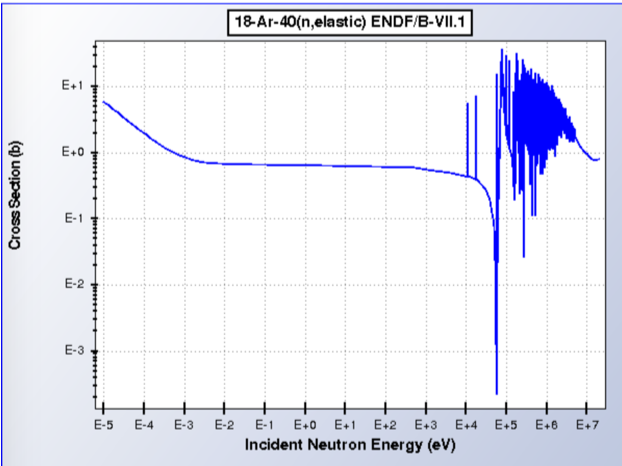
\includegraphics[width=0.4\linewidth]{Ar40xsec.png}
%\end{dunefigure}
%\fixme{Resolution of plots too bad and labels/titles not readable; get updated plots}

%\fixme{I don't find cit for ref:ENDF -anne}

The fixed, shielded deuterium-deuterium ($DD$) neutron generator would be located above a penetration in the hydrogenous insulation. Of order \SI{100}{$\mu$s} pulse width commercially available $DD$ generators exist that are about the size of a thermos bottle, and are cost competitive. Between the generator and the cryostat, layers of water or plastic and intermediate fillers will be included for sufficient degradation of the neutron energy. Initial simulations indicate that a single neutron injection point would illuminate the entire volume of one of the \dword{protodune} detectors and would be rapid (likely less than 30 min). 
%The $DD$ generator itself is the size of a large thermos bottle. 
%% KM repetitive with other part % Space needed by the system will be determined by the desired shielding level which is yet to be understood. 

The remaining studies for the TDR for the external neutron source include an assessment of the full design, including degrader materials and shielding and space and mounting (weight) considerations above the cryostat. Detailed simulation studies to understand the neutron transport process will be performed. In addition, the neutron capture gamma spectrum is also being characterized. In Nov 2017, the ACED Collaboration took several hundred thousand neutron capture events at the DANCE facility at LANSCE which will be used to prepare a database of the neutron capture gamma cascade chain. 
%from Vitaly, consider for future: I think a potential activation of materials due to this neutron source should be added to the remaining studies. Similarly, more detailed Monte Carlo of neutron transport to prove the concept of this calibration would help.
%KM can omit final detail if we need to.
%- do we need this detail here?} 
%\item Assessment of sufficient space and mounting (weight) considerations above the cryostat considering shielding for the neutron generator. 
%\end{itemize}

\subsection{External Muon Tracker} %1page
\label{sec:calibemt}

A external muon tracker (EMT), a dedicated fast tracking system, would provide track position, direction, and time information independent of TPC and PDS systems.

Rock muons from beam interactions in the rock surrounding the cryostat have similar energy  and angular  spectrum as CC \numu 
events. A nominal design of the EMT would cover the front face of the detector (approximately $14\textrm{m} \times 12\textrm{m}$) to provide an estimate of the initial position, and the time for a subset of these events, independent of the TPC and PDS systems. A second, similarly sized panel, \SI{1}{\m} away from the cryostat would provide directional information. 
%Preliminary studies have shown that with about \num{100} rock muons (of the approximately \num{800} that will arrive in \num{1}~year) it is possible to detect a \num{1}\% bias in rock-muon track reconstruction, which can be modeled as an error in the drift velocity $v_d$, at about the \num{2}$\sigma$ level.  
Additional measurements are possible elsewhere in the detector if the system is portable; it could be positioned on top of the cryostat to capture (nearly downward-going) cosmic rays during commissioning, or positioned along the side for rock muon-induced tracks along the drift direction. The EMT  pixelization will be small enough that rock-muon statistics will allow  determination of the center of each pixel to the same resolution as that expected for the detector (roughly \SI{1}{\cm}). So, for example, even with \SI{50} one-\si{\cm}-sized pixels,  with about \num{1000} rock muons per year passing through the EMT, the achievable precision  on average  for the incident position (before subsequent multiple scattering) is about \SI{5}{\milli\m}. 

%The number of rock muons entering the front face of the cryostat is similar to the number of CC \numu event rate contained in the detector.  

%This is a critical test for reconstruction in the forward \SI{1}{\m} region of the detector, which can be compared with information from cosmic rays and other calibration sources.


%This assumes that the test integrates over all $x$ and $y$, as doing the test in segments of $x$ and $y$ reduces the usable statistics.  
%In addition to the pixelization that will constrain $x$, $y$, $z$, and $t$ for each track, placing a second, identical counter about \SI{1}{\m} upstream will allow a measurement of the rock muon direction as well.

%KM: %Redundant %A concern is how such a system will be surveyed. Unlike APA and CPA crossers, these events will depend only on the relative position of the EMT and the APA that observes the muon.  Not knowing these relative positions will compromise the precision of the measurement, and the error in such a survey could be misinterpreted as a reconstruction bias.

%\fixme{Remaining studies should be standalone, avoid text repetition. Check this here.}

The remaining studies for the EMT system prior to the TDR include continued study of the precision with which the EMT (including panels on the sides and bottom) can determine biases or other problems with the detector model. Optimization of EMT size and pixelization and possible cost-saving options including re-use of existing scintillators (e.g. MINOS) or counter systems (e.g. ProtoDUNE or SBN) will be investigated. The available space for the EMT around the cryostat needs more investigation. A plan for surveying the EMT relative to the APAs also needs to be developed, to be coordinated with the APA consortium; error in such a survey could be misinterpreted as a reconstruction bias. %Continuation of discussions with the DAQ consortium on EMT needs, although this will depend somewhat on the technology chosen.
%KM May 

%\begin{itemize}
%\item
%Continuation of  simulation studies of the precision with which the EMT (including panels on the sides and bottom) can determine biases or other problems with the detector model. 
%\item Continuation of size and pixelization optimization. 
%\item Assessment of  space surrounding the cryostat for the EMT, including space above (for cosmic rays), along the side, or for a second panel \SI{1}{\m} away from the front face of the cryostat.
%\item Assessment of cost saving options, including reuse of existing scintillators (from MINOS), or reuse of a counter system (e.g., from \dword{protodune}).
%\item A plan for surveying the EMT relative to the APAs also needs to be developed, to be coordinated with the APA consortium; error in such a survey could be misinterpreted as a reconstruction bias.
%\item Continuation of discussions with the DAQ consortium on EMT needs, although this will depend somewhat on the technology chosen.
%\end{itemize}
%\fixme{SG: done reviewing until here. Need to take a break. }

%It would be good to add two sentences about DAQ stuff for all systems perhaps under summary. It could be as simple as we are trying understand DAQ requirements and I think we can say wehave some preliminary estimates nad refer to the table that went into the DAQ TP chapter?}

\subsection{Configuration of Proposed Systems} %1 page
\label{sec:FTs}

The current cryostat design for the 
\spmod with multi-purpose cryostat penetrations for various sub-systems is shown in Figure~\ref{fig:ftmap}. The penetrations dedicated for calibrations are highlighted in black circles. The placement of these penetrations is largely driven by the ionization track laser and radioactive source system requirements but would be usable for the neutron system as well.  The ports that are closer to the center of the cryostat are placed near the APAs (similarly to what is planned for SBND) to minimize any risks due to the \dword{hv} discharge. For the far east and west ports, \dword{hv} is not an issue as they are located outside the \dword{fc} and the penetrations are located near mid-drift to meet radioactive source requirements. 
%The multipurpose ports on far east and far west are located outside the field cage; the penetrations on the far east and west can  be used both by laser and radioactive source deployment systems. 

%In addition to these dedicated ports, the Detector Support System (DSS) and cryogenic ports (orange and blue dots in Figure~\ref{fig:ftmap}, respectively) will also be used as needed to route cables for the single phase photon detector calibration system. The DSS and cryogenic ports are accommodated with feedthroughs with a CF63 side flange for this purpose.   

\begin{dunefigure}[Top view of the \dword{spmod} 
cryostat showing various penetrations]{fig:ftmap}{Top view of the \dword{spmod} 
cryostat showing various penetrations. Highlighted in black ovals are multi-purpose calibration penetrations. The orange dots are TPC signal cable penetrations. The blue ports are \dword{dss} penetrations. The orange ports are TPC signal cable penetrations. The larger purple ports at the four corners of the cryostat are human access tunnels.}
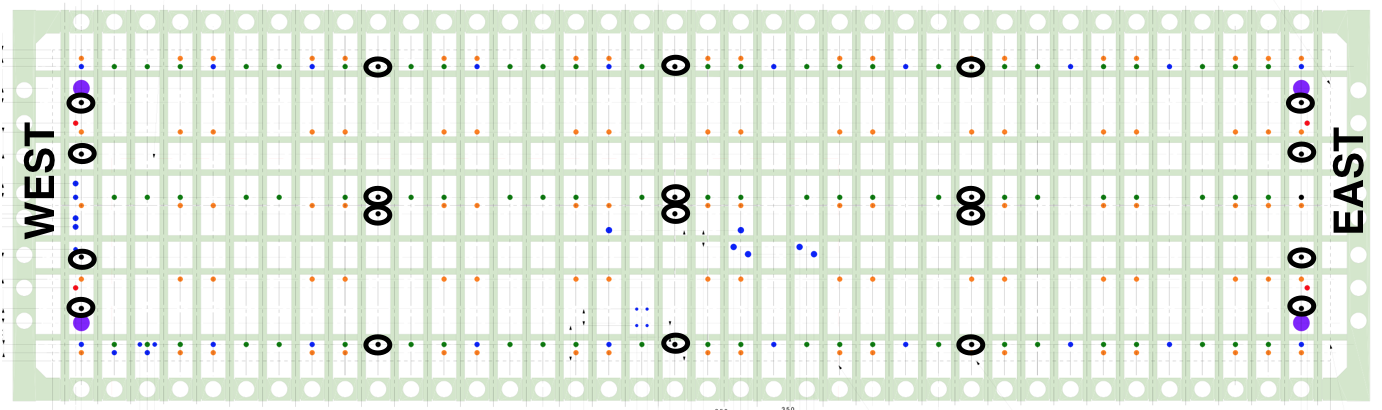
\includegraphics[height=2.0in]{FTmap.png}
\end{dunefigure}


Implementation of the ionization laser system, proposed in Section~\ref{sec:laser}, requires 20 feedthroughs to cover the four TPC drift volumes; this arrangement would provide (almost) full volume calibration of the electric field and associated diagnostics (e.g. HV). The crossing laser tracks are necessary to unambiguously construct the field map. A steerable plastic insulator laser head and fiber interface would be mounted on top of the cryostat in the feedthrough. Two options are under investigation: (1) the \dword{fc} (but not the ground plane or the active volume) is penetrated, and (2) the \dword{fc} is not penetrated. In the former case, the \dword{fc} penetration has been shown to create a small distortion to the \efield, for the benefit of full volume \efield mapping. When the \dword{fc} is not penetrated, the laser shines through the \dword{fc} tubes, producing some regions that are not mappable by the laser, and it will not be possible to map the position of the track start making the analysis more difficult. This is the case for laser system which use the far east and west ports. The necessity of penetrating the \dword{fc} has not been fully assessed yet. The \phel system would employ fixed fibers, and would not require a steering mechanism or mechnical FC penetrations.

The distance between any two consecutive feedthrough columns in Figure~\ref{fig:ftmap} is about \SI{15}{\m}, a plausible distance for the laser beam to travel. The maximum distance light would travel to the bottom corner of the detector, would be approximately \SI{20}{\m}.  Direct-ionization tracks have been demonstrated at a maximum possible distance in \microboone of \SI{10}{\m}. The Rayleigh scattering of the laser light is about \SI{40}{\m}, but additional optics effects, including self-focusing (Kerr) effects may limit the maximum practical range. Assuming these are not a limitation, this laser arrangement could illuminate the full volume with crossing track data. It is important to note that at this point in time, a maximum usable track length is unknown and it is possible that the full \SI{60}{\m} \detmodule length could be achieved by the laser system after optimization.

The calibration group focused on finalizing the cryostat penetrations for the \spmod driven by the cryostat design timeline. A similar exercise will be done to finalize \dpmod penetrations for calibrations in the near future.

